\chapter{Ground Truth Generaiton: ArUco Markers and Plane Fitting (Refined Approach)}

\section{Introduction}
To overcome the limitations of the initial ellipse fitting 
approach, a second method was developed using ArUco markers and 
plane fitting. This method aimed to achieve precise 3D 
estimation of the steering wheel's location and orientation. 
The use of ArUco board, and a plane fitting technique allowed 
for a more robust and accurate approach to capturing the 3D 
geometry of the steering wheel. By leveraging the known 
properties and spatial relationships of the ArUco markers, 
this refined method was able to provide a reliable and 
high-quality ground truth for the steering wheel's position 
and orientation, which could then be used for training and 
evaluating 3D object detection models.


ArUco markers \cite{opencv_aruco_detection} are widely used  in 
computer vision for precise localization and pose estimation 
tasks.  An ArUco marker as depicted in \cref{fig:marker}, is a 
synthetic square marker featuring a  thick black border and an 
inner binary matrix that encodes  its identifier (ID). The black 
border enables quick detection  in images, while the binary 
matrix allows for identification  and supports error detection 
and correction.  The marker size dictates the dimensions of the 
internal matrix;  for example, a 4x4 marker contains 16 bits. 
can be easily  detected and identified in images.  They offer 
several advantages, including robustness to  variations in 
lighting, simple detection with minimal  computational overhead, 
and compatibility with popular  libraries like OpenCV, which 
provides dedicated functions for detecting ArUco markers and 
estimating their pose in both 2D  and 3D. Figures \cref{fig:marker_detection} and \cref{fig:marker_orientation} 
demonstrate OpenCV's capabilities in detecting ArUco markers and 
estimating their 3D position, respectively. 

This chapter presents the structured methodology, the evaluation 
of different techniques for location and orientation estimation, 
and the results of this second approach in accurately capturing 
the steering wheel’s 3D geometry.

\begin{figure}[ht]
    \centering
    \begin{subfigure}[t]{0.3\textwidth}
        \centering
        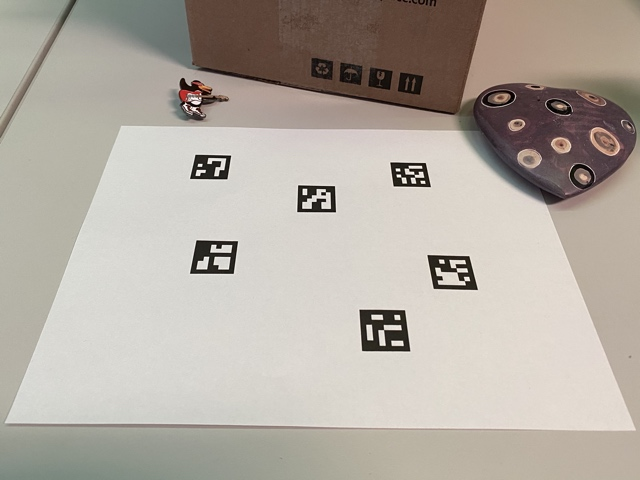
\includegraphics[width=\textwidth]{media/chapter 5/singlemarkersoriginal.jpg}
        \caption{Single ArUco Markers}
        \label{fig:marker}
    \end{subfigure}\hfill
    \begin{subfigure}[t]{0.3\textwidth}
        \centering
        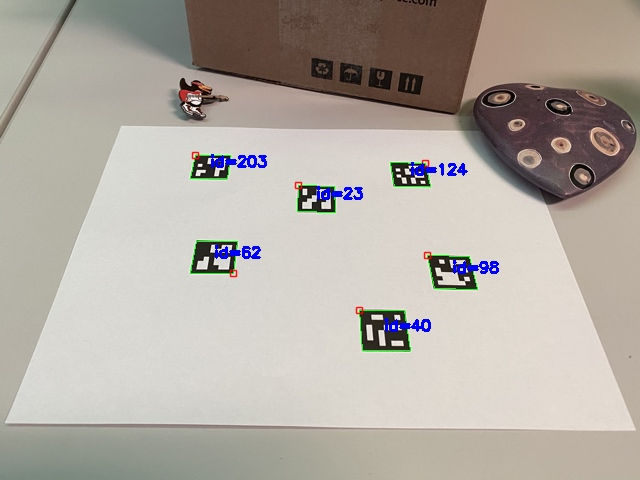
\includegraphics[width=\textwidth]{media/chapter 5/singlemarkersdetection.jpg}
        \caption{These are the detected markers (in green). 
        Note that some markers are rotated. 
        The small red square indicates the marker’s top left 
        corner}
        \label{fig:marker_detection}
    \end{subfigure}\hfill
    \begin{subfigure}[t]{0.3\textwidth}
        \centering
        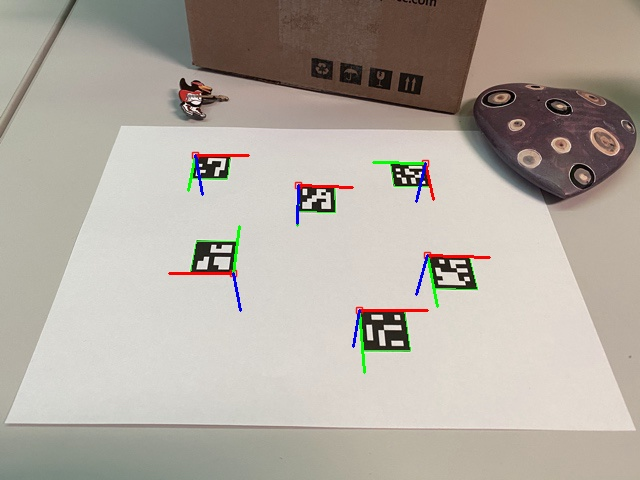
\includegraphics[width=\textwidth]{media/chapter 5/singlemarkersaxes.jpg}
        \caption{The marker coordinate system that is placed in the center or in the top left 
        corner of the marker with the Z axis pointing out. 
        Axis-color correspondences are X: red, Y: green, Z: blue.}
        \label{fig:marker_orientation}
    \end{subfigure}
    \caption{ArUco merkers' detection and pose estimation by OpenCV.}
\end{figure}

This refined approach aimed to address the challenges 
encountered in the initial method, particularly the issues of 
data sparsity, noise, and inaccurate geometric representation. 
By leveraging the advantages of ArUco markers, this method 
sought to tackle the difficulties in precisely estimating the 
3D position and orientation of the steering wheel. 

The proposed technique involved positioning a board with 
multiple ArUco markers at the center of the steering wheel 
like in \cref{fig:gt_stream} and employing plane fitting to 
enhance the accuracy of orientation estimation. 
This approach was extensively evaluated to validate its 
reliability in capturing the 3D geometry of the steering wheel.

The following sections detail 
the assessment of ArUco markers for location and orientation 
estimation, as well as the generation of the steering wheel's 
oriented bounding box using the validated methods.

\section{Methodoloy}
To address the limitations identified in the initial approach, 
a structured methodology was developed using ArUco markers and 
plane fitting. The ArUco markers were placed on a board mounted 
at the center of the steering wheel as depicted in 
\cref{fig:gt_stream}. This setup allowed us to capture both the 
2D and 3D spatial data required for accurately estimating the 
steering wheel's position and orientation.

The methodology involved two primary components for estimating 
the location and orientation of the steering wheel. 
each component is described in detail in the following 
subsections:

\subsection{location estimation}
As depicted in \cref{fig:gt_stream}, the ArUco board is positioned at the center of the steering 
wheel. Therfore, the detected centroid of the ArUco board directly 
corresponds to the 3D spatial coordinates of the steering 
wheel's center. Given the known arrangement of markers on the 
ArUco board, the location of the board's center, and 
consequently the steering wheel's center, can be readily 
inferred from the detected positions of the individual markers.

To achieve precise location estimation of the ArUco markers, 
we considered two primary approaches:

\textbf{1. Direct 3D Estimation Using OpenCV: }
OpenCV’s \emph{estimatePoseSingleMarkers} function provides a direct 
way to estimate the 3D position of markers relative to the camera. 
This function relies on the known physical size of the 
ArUco markers and the intrinsic camera parameters to calculate 
the translation vector, which represents the 3D position of 
the markers as [dx, dy, dz] where dx dy, and dz are the marker's 
position along the x, y, and z axes, respectively. 
While this method offers a straightforward approach, its 
accuracy can be sensitive to marker orientation, distance from 
the camera, and the angle of view.

\textbf{2. 2D Estimation with Mapping to 3D: }
This alternative method starts by detecting the 2D position of 
the markers in the image plane using OpenCV’s \emph{detectMarkers} 
function. \Cref{fig:detectMarkers} shows merkers' location detected 
by OpenCV on the 2D image.
After detecting the 2D positions, these points are 
mapped to 3D space using depth information derived from the 
point cloud data and the camera’s intrinsic parameters. 
This approach separates the detection process into two stages, 
potentially improving accuracy by isolating the detection of 
2D marker positions from their 3D mapping.
\begin{figure}[ht]
    \centering
    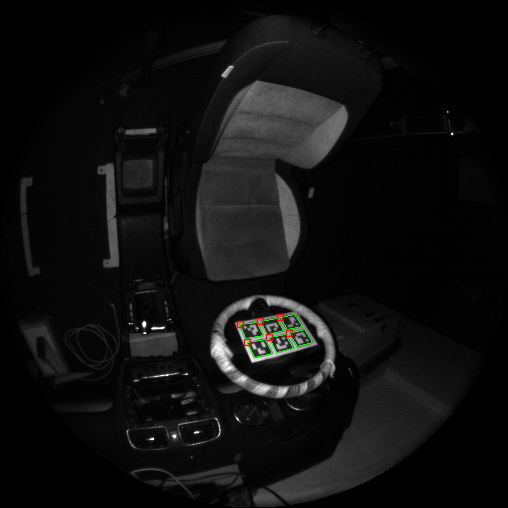
\includegraphics[scale=0.5]{media/chapter 5/aruco_detection.png}
    \caption{OpenCV detected the ArUco markers' location in the 2d image.}
    \label{fig:detectMarkers}
\end{figure}


Given the known structure and location of the markers on the board, 
we employed a method to calculate the board’s center based on the 
spatial relationship of specific marker pairs. This technique ensured 
that the center could be reliably calculated even if some markers were 
undetected.

To calculate the center of the board, we utilized three pairs of markers 
that are symmetrically positioned on opposite sides of the board as depicted
in \cref{fig:marker_ids}. These marker pairs are: \{(0, 5), (1, 4), (2, 3)\}

For each detected pair, the midpoint between the two markers was 
computed by averaging their translation vectors \( tvec \), which 
represent the 3D coordinates of each marker. This midpoint provides an 
estimate of the board’s center based on that particular pair.

For each detected pair \((i, j)\), we compute the midpoint as:
\[
\text{midpoint}_{ij} = \frac{tvec_i + tvec_j}{2}
\]

where  \(tvec_i\)  and  \(tvec_j\)  are the translation vectors 
(3D coordinates) of markers  \(i\)  and  \(j\) . Once the midpoints for 
all detected pairs are obtained, the overall center of the board is 
calculated as the mean of these midpoints:

\[
\text{center}_\text{board} = \frac{\sum{(i, j) \in \text{detected pairs}} \text{midpoint}_{ij}}{N}
\]

where  \(N\)  is the number of detected pairs. The resulting averaged 
translation vector represents the estimated 3D center of the board. 


By considering the relative positions and midpoints of detected marker 
pairs, this method can robustly determine the center point of the board, 
providing an accurate 3D location for the steering wheel despite 
potential occlusions or missing markers.

\begin{figure}[ht]
    \centering
    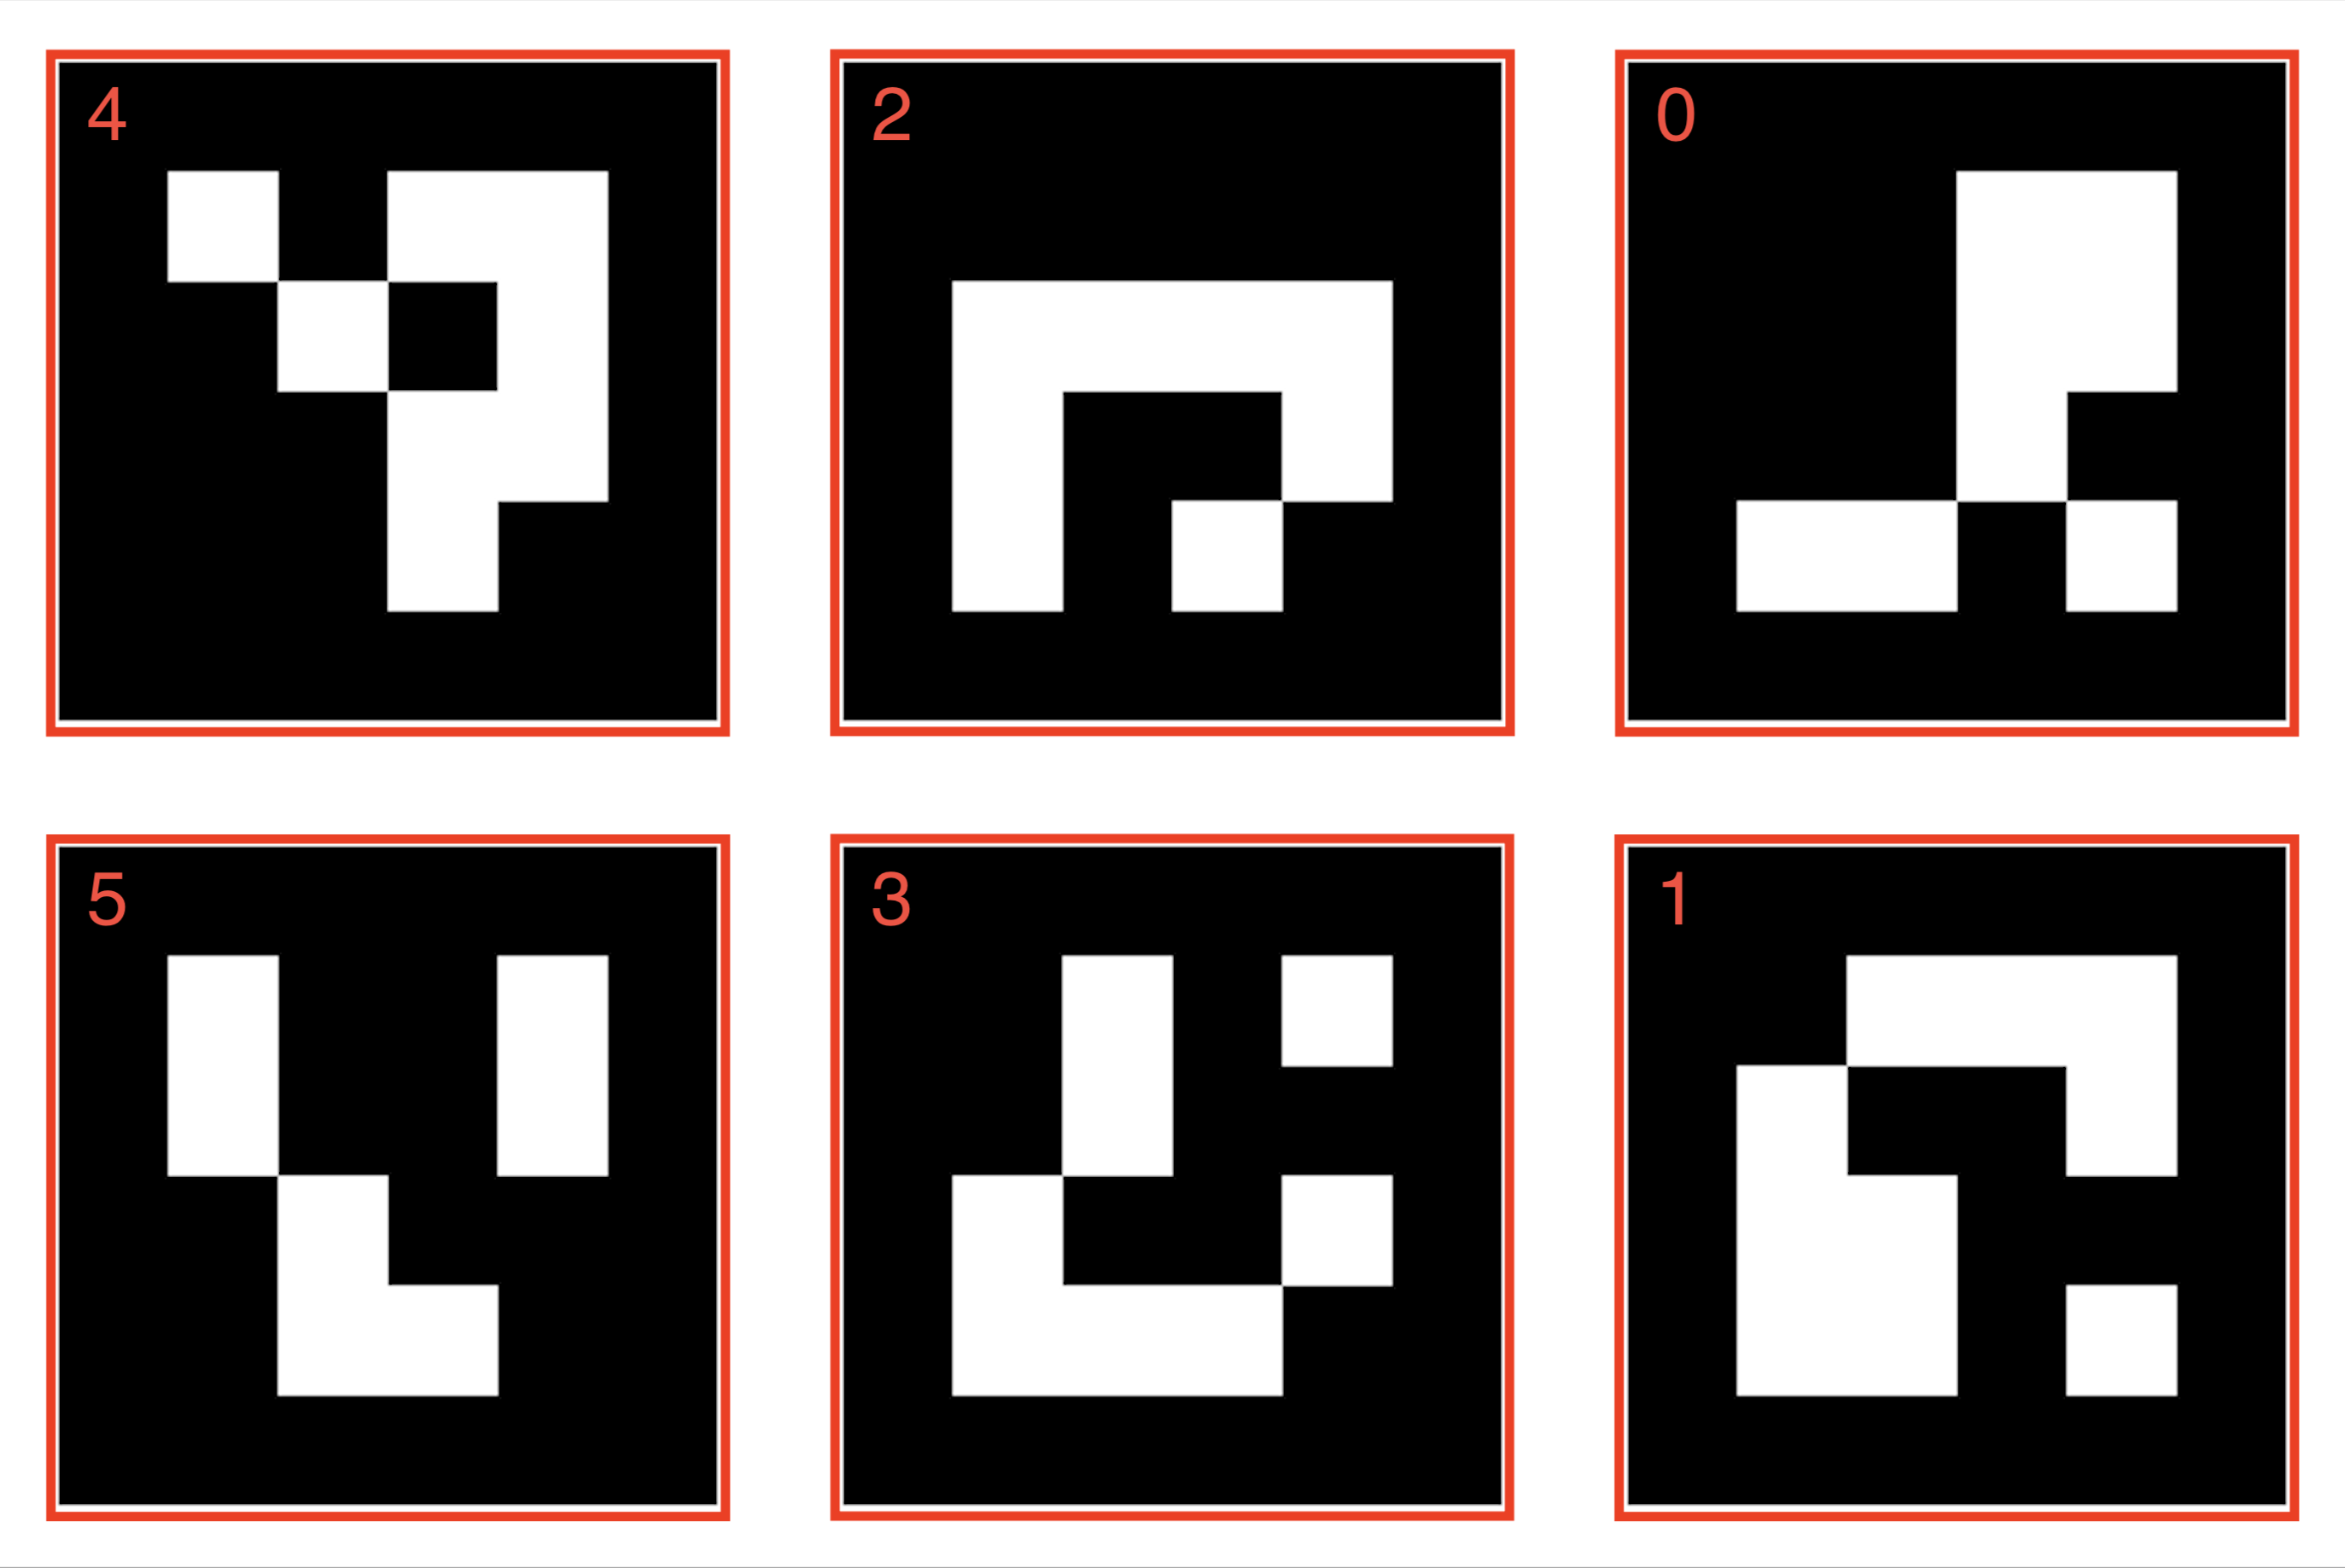
\includegraphics[scale=0.5]{media/chapter 5/aruco_board_ids.png}
    \caption{To calculate the center of the board, we utilized multiple 
    marker pairs that are symmetrically positioned on opposite sides of 
    the board as marker pairs \{(0,5), (1,4), (2,3)\}.}
    \label{fig:marker_ids}
\end{figure}


\subsection{Evaluating ArUco Markers for Orientation Estimation}
Accurately determining the orientation of the marker board was 
critical for estimating the steering wheel’s orientation. 
As the ArUco board is accurately placed tangent to the steering 
wheel, the orientation of the board corresponds to the 
orientation of the steering wheel in 3D space. 

Two methods were used exploited to estimate the orientation of 
the ArUco board: 

\uzlemph{Direct Orientation Estimation Using OpenCV: }
OpenCV’s \emph{estimatePoseSingleMarkers} function also calculates the 
orientation of markers in the form of rotation vectors. 
These vectors indicate the rotational pose of each marker 
relative to the camera’s coordinate system. Assuming the we 
know the  orientation of the markers on the board, we can 
remove the outlier markers and average the remaining rotation 
vectors to estimate the overall orientation of the board.
However, this method has limitations, as it relies on the 
accuracy of OpenCV's built-in pose estimation.

As illustrated in \cref{fig:estimatePoseSingleMarkers}, 
OpenCV's estimations of marker 
positions on a 3×4 board are highly sensitive to several factors. 
These include the camera angle, the distance of the markers from 
the camera, occlusion of the markers, and other environmental 
factors. Consequently, when markers are missing or occluded, 
the reliability and accuracy of the orientation estimation can 
decrease significantly. This sensitivity to various spatial and 
environmental conditions highlights the limitations of relying 
solely on OpenCV's built-in pose estimation functions for robust 
3D orientation determination.

\begin{figure}[ht]
    \centering
    \begin{subfigure}[t]{0.23\textwidth}
        \centering
        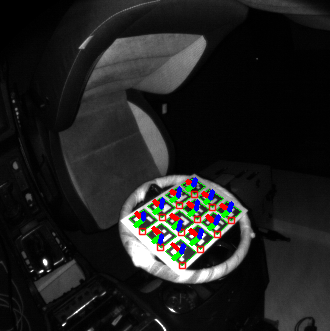
\includegraphics[width=\textwidth]{media/chapter 5/aruco_board_estimation0.png}
    \end{subfigure}\hfill
    \begin{subfigure}[t]{0.23\textwidth}
        \centering
        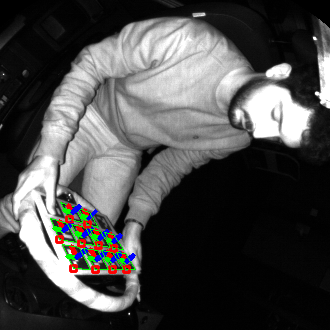
\includegraphics[width=\textwidth]{media/chapter 5/aruco_board_estimation1.png}
    \end{subfigure}\hfill
    \begin{subfigure}[t]{0.23\textwidth}
        \centering
        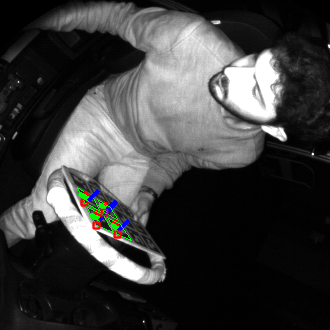
\includegraphics[width=\textwidth]{media/chapter 5/aruco_board_estimation2.png}
    \end{subfigure}\hfill
    \begin{subfigure}[t]{0.23\textwidth}
        \centering
        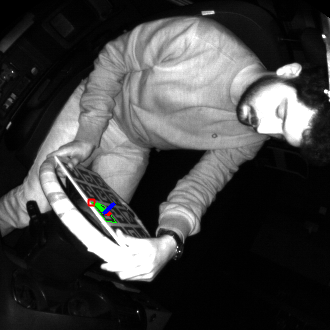
\includegraphics[width=\textwidth]{media/chapter 5/aruco_board_estimation3.png}
    \end{subfigure}
    \caption{The markers' coordinate system estimated by OpenCV's
            \emph{estimatePoseSingleMarkers} function on a 3x4
            board shows that this method is highly sensitive
            to the markers' distance, camera angle and other
            environmental factors. Axis-color correspondences are 
            X: red, Y: green, Z: blue, with Z axis pointing out}
    \label{fig:estimatePoseSingleMarkers}
\end{figure}

\uzlemph{Plane Fitting Method: }
The plane fitting method provided a more robust and reliable 
means of estimating the orientation, as it doesn't depend solely 
on the accuracy of OpenCV's pose estimation for individual 
markers. This approach overcomes the limitations of the direct 
orientation estimation using OpenCV, which can be sensitive to 
factors like marker size, distance, and viewing angle. 
Hence, the plane fitting method offers a more stable and 
accurate estimate of the steering wheel's orientation under a 
variety of conditions.

This method involves the following steps:

\begin{enumerate}
    \item \emph{Finding the Center of the ArUco Board: }
    To initiate plane fitting, it is essential to first locate 
    the center of the ArUco board. This is done using the 
    detected marker locations. Given that the markers are 
    arranged in a known, fixed structure on the board, 
    the center can be reliably estimated even if one or more 
    markers are not detected. By analyzing the relative 
    positions of the detected markers, the center of the board 
    can be computed with high accuracy.
    \item \emph{Sampling Points Around the Center: }
    Once the center of the ArUco board is determined, 
    a set of points is sampled from the board around this 
    central point within a specified radius. This sampling 
    process ensures that the points used for plane fitting are 
    well-distributed across the board, enhancing the reliability 
    of the orientation estimation. \Cref{fig:plane_fitting} shows 
    the sampled points from the board in red.
    \item \emph{Fitting a Plane to the Sampled Points: }
    The sampled points are then used to fit a plane. 
    The fitting process involves computing the best-fit plane 
    that minimizes the distance between the plane and the 
    sampled points. This plane effectively represents the 
    overall orientation of the ArUco board.
    \item \emph{Using the Normal Vector for Orientation: }
    The normal vector of the fitted plane is then calculated. 
    This normal vector serves as a robust indicator of 
    the board’s orientation in 3D space. As \cref{fig:plane_fitting}
    shows, the light blue line indicated the norm vector of the board.
    Since the board is mounted on the steering wheel tangent to the 
    steering wheel's surface, the orientation of this normal vector 
    directly corresponds to the orientation of the steering wheel.
\end{enumerate}

\begin{figure}[ht]
    \centering
    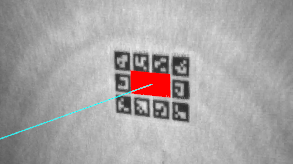
\includegraphics[width=0.5\textwidth]{media/chapter 5/plane_fitting.png}
    \caption{Illustration of the plane fitting method, showing the 
    sampled points around the center of the ArUco board in red and the 
    normal vector of the fitted plane in light blue, which represents 
    the orientation of the steering wheel.}
    \label{fig:plane_fitting}
\end{figure}

One of the significant advantages of this method is its 
robustness to marker detection failures. Even if some markers 
are not detected due to occlusions, lighting conditions, or 
other factors, the known arrangement of the markers allows for 
accurate estimation of the board’s center and subsequent 
orientation. This makes the plane fitting method highly 
resilient to errors in individual marker detections, ensuring 
reliable orientation estimation under a variety of conditions.


\subsection{Generating the Steering Wheel’s Oriented Bounding Box}
\section{Results}
\subsection{Location Estimation Results}
\uzlemph{Inter-Marker Distance Evaluation}
\uzlemph{Distance and Angle Variation}
\subsection{Orientation Estimation Results}
\
\subsection{Systematic Error in Orientation Estimation}
\subsection{Generating the Steering Wheel’s Oriented Bounding Box}

\section{Conclusion}